% Created 2023-04-23 Sun 17:48
% Intended LaTeX compiler: pdflatex
\documentclass[twocolumn]{article}
\usepackage[utf8]{inputenc}
\usepackage[T1]{fontenc}
\usepackage{graphicx}
\usepackage{longtable}
\usepackage{wrapfig}
\usepackage{rotating}
\usepackage[normalem]{ulem}
\usepackage{amsmath}
\usepackage{amssymb}
\usepackage{capt-of}
\usepackage{hyperref}
\usepackage{balance}
\usepackage{graphics}
\usepackage{txfonts}
\usepackage{times}
\usepackage{color}
\usepackage{textcomp}
\usepackage{booktabs}
\usepackage{todonotes}
\usepackage{float}
\usepackage{url}
\usepackage{titling}
\usepackage[left=3cm,right=2cm,top=2.5cm,bottom=2cm]{geometry}
\usepackage[british]{babel}
\usepackage{placeins}
\usepackage{stfloats}
\usepackage[ruled, lined, linesnumbered, commentsnumbered, longend]{algorithm2e}
\newcommand{\Mod}[1]{\ (\mathrm{mod}\ #1)}
\usepackage{sectsty}
\sectionfont{\Large}
\subsectionfont{\large}
\subsubsectionfont{\large}
\paragraphfont{\normalsize}
\setlength{\parindent}{0em}
\setlength{\parskip}{1em}
\setlength{\columnsep}{2em}
\setlength{\droptitle}{-5em}
\makeatletter
\def\url@leostyle{%
\@ifundefined{selectfont}{\def\UrlFont{\sf}}{\def\UrlFont{\small\bf\ttfamily}}}
\makeatother
\urlstyle{leo}
\usepackage[
%backend=biber,
natbib=true,
style=numeric,
sorting=none
]{biblatex}
\addbibresource{/home/struan/Documents/University/Dissertation/library.bib}
\addbibresource{/home/struan/Sync/library.bib}
\author{Struan Robertson \\ BSc (Hons) Applied Computing}
\date{May 2023}
\title{Terrain Model Processing with Machine Learning}
\hypersetup{
 pdfauthor={Struan Robertson \\ BSc (Hons) Applied Computing},
 pdftitle={Terrain Model Processing with Machine Learning},
 pdfkeywords={},
 pdfsubject={},
 pdfcreator={Emacs 28.2 (Org mode 9.6.1)}, 
 pdflang={English}}
\begin{document}

\maketitle
\begin{abstract}

With the launch of the lunar orbiter laser altimeter (LOLA) on NASA's lunar reconnaissance orbiter (LRO), a large amount of high-resolution digital elevation maps (DEMs) have been constructed, providing a precise topographical model of the moons surface.
These DEMs are prone to voids containing no data, making the map less reliable for scientific purposes and future moon missions.
This paper uses a machine learning model to allow for the technique of image inpainting to be used with lunar DEMs.
Image inpainting uses pixel data from an image to generate missing data to fill a void.
DEMs can be thought of mathematically as identical to a single channel (greyscale) image, a two-dimensional array with "pixel" values corresponding to height, and so the technique of image inpainting can be easily applied to DEMs.
A Generative Adversarial Network (GAN) based on a fully convolutional architecture was used for the inpainting.


\end{abstract}

\section{Introduction}
\label{sec:org6e1f7b9}

Sensory data from the Lunar Orbiter Laser Altimeter (LOLA) and Lunar Reconnaissance Orbiter Camera (LROC) has been used for the construction of Lunar digital elevation models (DEMs) since the launch of the Lunar Reconnaissance Orbiter (LRO) in 2009.
LRO has several primary objectives as part of a series of robotic missions that aim to pave the way for a permanent human presence on the Moon, including determining the global topography of the lunar surface at meter-scale resolution.
Topographical data from LOLA and LROC will be used to facilitate the selection of future landing sites, so accuracy and completeness are essential.
\autocite{chinLunarReconnaissanceOrbiter2007}

The LRO is in a polar orbit around the moon, scanning the surface in swathes 50 to 60m wide, with an average separation ranging between 1.2km and 200m depending on the position of LRO in orbit.
LOLA uses a laser altimeter to measure the distance from LRO to the lunar surface at 5 different spots simultaneously, providing DEMs ranging from \textasciitilde{}30m resolution at the equator to \textasciitilde{}5m resolution at the poles. \autocite{smithLunarOrbiterLaser2010}.
LROC uses two narrow-angle cameras (NACs) to collect stereo observations at a resolution of 0.5 to 1.5 m per pixel.
These high resolution images can be used to generate high resolution (\textasciitilde{}5m at the equator) DEMS, referred to as NAC DEMs \autocite{tranGeneratingDigitalTerrain2010}.

Both LOLA and NAC dems are prone to no-data voids resulting from shadowed regions (NAC) or terrain features blocking the return of the laser altimeter (LOLA).
As the LRO has a polar orbit, data is recorded in strips, which must be joined together to create larger DEMs. These strips are not immediately adjacent to each other, resulting in a no-data void in-between.
Reconstructing these no-data voids is non-trivial, with Park and Choi \autocite{parkNeuralProcessApproach2021}  noting the following challenges:
\begin{itemize}
\item NAC DEMs require high-resolution reconstruction methodology
\item NAC DEMs are large and high-resolution area maps, thus a scalable approach should be applied
\item The reconstruction algorithm must be reliable since it can affect related lunar studies or exploration missions
\end{itemize}

Traditional algorithmic methods for correcting no-data voids within DEMs include inverse distance weight method (IDW), local polynomial interpolation method (LPI), spline with tension method (ST) and other algorithms to interpolate the elevation sampling points. Interpolation methods use the neighboring elevation values for void infilling, thus performance is directly proportional to the size of the void.
Voids of any significant size result in interpolation methods returning inaccurate reconstruction results.  \autocite{reuterEvaluationVoidFilling2007}

Within the field of computer vision, the problem of image inpainting fundamentally seeks to solve the same issue as DEM void infilling; a 2-dimensional grid of points with an area of no data which must be inferred from surrounding points.
RGB images contain three channels whereas a DEM contains only one, however inpainting techniques process each channel independently and then combine the results, so inpainting a DEM is functionally identical to inpainting a greyscale image.
Generative adversarial networks (GANs)\autocite{goodfellowGenerativeAdversarialNetworks2020} are a deep learning generative model that when constructed with deep convolutional neural networks\autocite{krizhevskyImageNetClassificationDeep2017} have been shown to have excellent performance in image inpainting\autocite{pathakContextEncodersFeature2016,yuGenerativeImageInpainting2018} and have been successfully applied to the task of DEM void infilling\autocite{gavriilVoidFillingDigital2019,zhangVoidFillingBased2020,qiuVoidFillingDigital2019}.

This papers implements a GAN inpainting network based on the structure described by Yu \emph{et al.}\autocite{yuGenerativeImageInpainting2018} and shows it to effectively pass the first two challenges set forward by Park and Choi.
The final challenge of DEM reliability may be passed by this network, however this is difficult to test as GANs excel at infilling \emph{plausible} data, yet the \emph{accuracy} of this data may not be necessarily sufficient.


\section{Background}
\label{sec:orga3d8ad1}
\subsection{Digital Elevation Maps}
\label{sec:org5f0ecfa}

Digital elevation maps (DEMs) are digital representations of terrain elevation (Figure \ref{fig:apollo_17}).
A DEM consists of a grid of cells, where each cell represents a specific area of terrain and contains the elevation value of the ground at this location.
The cells of a DEM can also be described as pixels, as they represent a discrete location in a raster grid.
DEM gridsize refers to the size of cells and can be thought of as the resolution of the DEM.
Gridsize can vary depending on the source of data and the intended application, with common grid sizes ranging from a few meters to several kilometers.

\begin{figure}[htbp]
\centering
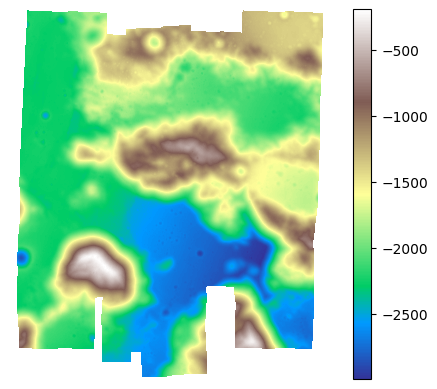
\includegraphics[width=.9\linewidth]{images/apollo_17.png}
\caption{\label{fig:apollo_17}Shaded DEM of Apollo 17 landing site in Taurus-Littrow Valley}
\end{figure}

\begin{figure}[htbp]
\centering
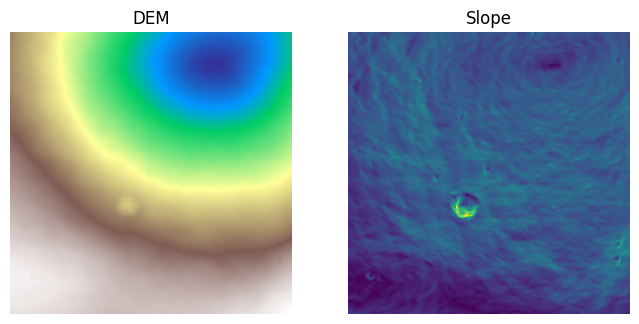
\includegraphics[width=.9\linewidth]{images/dem_and_slope.png}
\caption{\label{fig:dem_and_slope}Section of DEM with computed slope}
\end{figure}

The slope of a DEM refers to the steepness of terrain at each location in the map (Figure \ref{fig:dem_and_slope})
Slope is calculated by traversing a 3 x 3 window (Figure \ref{fig:window}) over the DEM\autocite{qiuVoidFillingDigital2019}.
The slope value at the central pixel \emph{e} can be calculated by using the algorithm proposed by Horn \emph{et al.}\autocite{hornHillShadingReflectance1981} :
\begin{align}\label{eqn:slope}
Slope &= arctan\sqrt{Slope^2_{we} + Slope^2_{sn}}, \\
Slope_{we} &= \frac{(e_8 + 2e_1 + e_5) - (e_7 + 2e_3 + e_6)}{8 \times Gridsize}, \\
Slope_{sn} &= \frac{(e_7 + 2e_4 + e_8) - (e_6 + 2e_2 + e_5)}{8 \times Gridsize},
\end{align}

\begin{figure}[htbp]
\centering
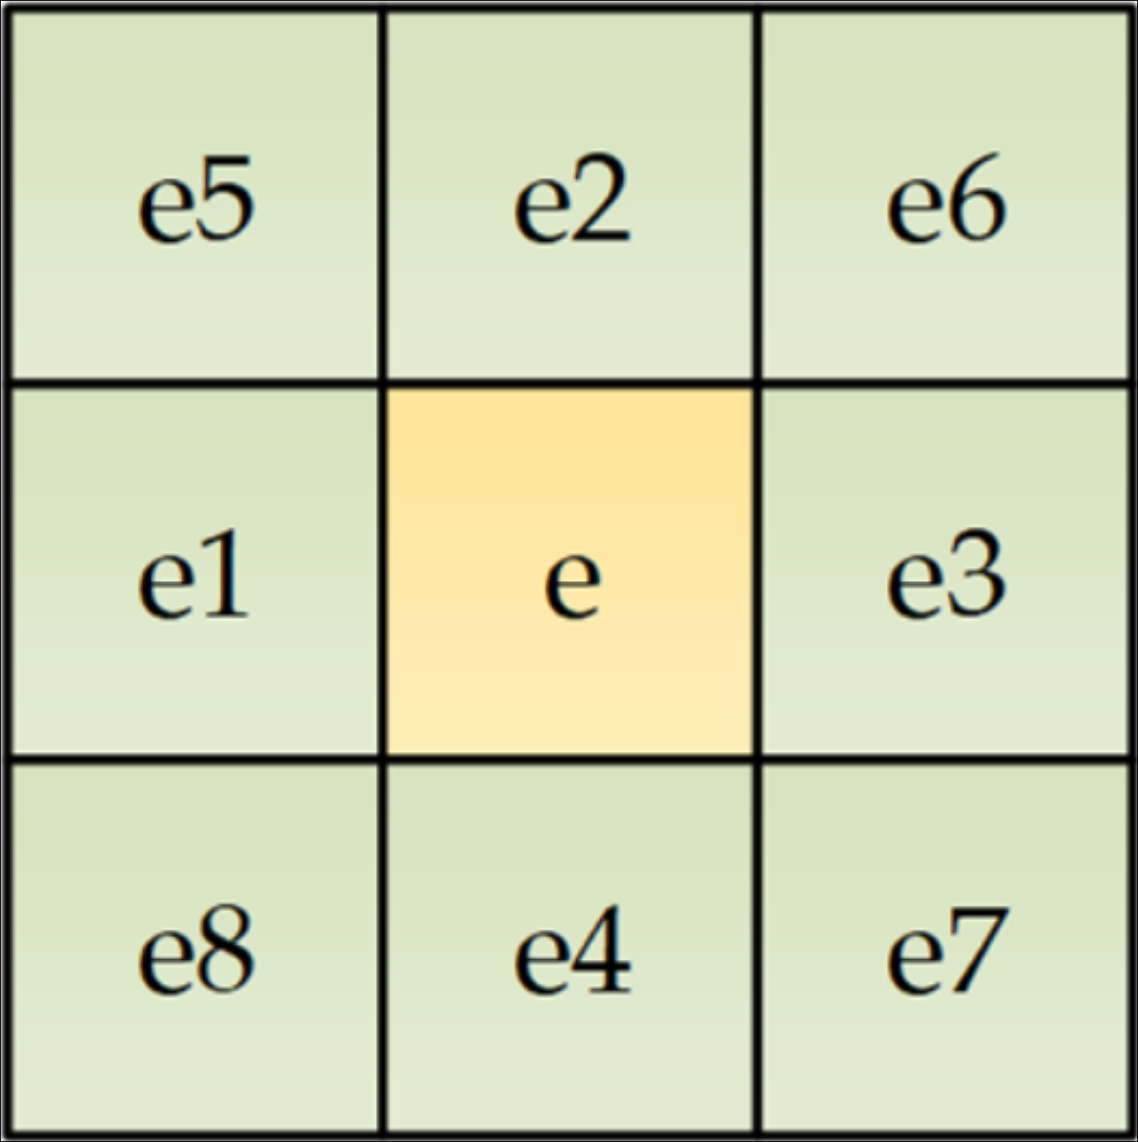
\includegraphics[width=4cm]{images/window.png}
\caption{\label{fig:window}The 3x3 moving window\autocite{qiuVoidFillingDigital2019}}
\end{figure}

The most common data format for the storage of DEMs is GeoTiff.
A GeoTiff is a type of TIFF (Tagged Image File Format) that with the raw DEM raster data also stores spatial metadata such as pixel resolution (gridsize).
Lunar DEMs are also commonly stored in NASA's PDS (Planetary Data System) archival formats PDS3 and PDS4.
PDS is used to archive multiple kinds of data from planetary science missions, not just DEMs.
Older missions (pre 2011) are typically archived in PDS3, with post 2011 missions using PDS4.
Although stored differently, the raster data in PDS files and GeoTiffs is identical.

The issue of no-data voids is not limited to lunar DEMs, as DEMs are typically constructed using remote sensing technology which is prone to the same errors.

\subsection{Deep Neural Networks}
\label{sec:orgdbf2a28}

Neural networks are a type of machine learning algorithm that is loosely modeled after the structure and function of biological brains, consisting of multiple artificial neurons\autocite{grossiIntroductionArtificialNeural2008}.
A neuron can hold any value, however in most neural networks this value is restricted between 0 and 1 or -1 and 1.
The value a neuron holds is referred to as its activation.
When data is passing forwards through a network, each neuron has an activation determined by the input data.
In a fully connected network, these neurons are arranged into layers, with every neuron in a layer connected to every neuron in the previous layer (Figure \ref{fig:neural_network}) .
The first layer is the input layer, the last the output layer and the layers in-between are hidden layers.
In image processing tasks, such as image inpainting, the neurons in the input layer correspond to the pixels of the input image.
The layered structure of the neural network is highly efficient as it allows the network to break down complex problems into smaller steps.

\begin{figure}[htbp]
\centering
\includegraphics[width=.9\linewidth]{images/neural_network.png}
\caption{\label{fig:neural_network}Simple feedforward artifical neural network\autocite{ArtificialNeuralNetwork2023}}
\end{figure}

Each connection between neurons in different layers has an associated weight.
This weight is an indication of how the neuron in the second layer is correlated to the neuron in the first.
A positive weight indicates that when the first neuron has a high activation so should the second, and a negative weight the inverse.
Each neuron also holds a value called a bias, which can be thought of as the minimum weighted sum for the neuron to activate.
To compute the activation of a second layer neuron, take the sum of the activations of the first layer neurons multiplied with their weights and add the bias (Equation \ref{eqn:activation}).
The activation can be any number, however to normalise the signal between a range and add non-linearity to the network the activation is passed through an activation function.

ReLU (Rectified Linear Unit) is an activation function which can introduce sparsity into the network, meaning only a subset of neurons will be activated for any given input.
The constant gradient of ReLU when the gradient is positive improves the stability of gradients in the network, making vanishing gradients less likely than other activation functions, such as sigmoid.
ReLU also introduces sparsity in the activations since it outputs zero for negative input values.
Whilst this can simplify the network and reduce computational complexity, it can also lead to the "dying ReLU" problem, where some neurons in the network stop contributing to the output due to always receiving negative input values and having an output of zero.
The ELU activation function (Figure \ref{fig:ELU}) becomes smooth slowly until its output equals \(-\alpha\) for negative inputs, ensuring all neurons in the network can contribute to the output even if their inputs are negative.
This can improve the performance of the network when dealing with noisy or outlier data, which is very common in DEMs.
For this reason ELU is the most common activation function in the network described by this paper.
Other activation functions used are Leaky ReLU and Tanh.
Leaky ReLU also addresses the dying ReLU problem, however instead of a smooth curve to \(-\alpha\), negative values have a small constant negative slope equal to \(\alpha\) (usually 0.1).
Leaky ReLU is used in the critic of this the network described by this paper as it allows the activation to be infinitely small.
In generative networks such as the generator, this can lead to vanishing gradients, however in classifier networks such as the critic it is important for it to be able to learn negative associations.
The Tanh activation function compresses all activations to between -1 and 1, and so is used as the final layer in generative networks to produce output data of the same range as the input data.

\begin{equation}
\label{eqn:activation}
a^{(1)}_0 = ELU(w_{0,0}a^{(0)}_0 + w_{0,1}a^{(0)}_1 + \cdots + w_{0,n}a^{(0)}_n + b_0)
\end{equation}

\begin{figure}[htbp]
\centering
\includegraphics[width=.9\linewidth]{images/ELU.png}
\caption{\label{fig:ELU}ELU activation function}
\end{figure}


As the equations are linear, to efficiently compute the activation of every neuron in a forward layer, the equations can be stacked into matrices\autocite{3Blue1BrownWhatNeural} :
\begin{equation}
\begin{bmatrix} a^{(1)}_0 \\ a^{(1)}_1 \\ \vdots \\ a_n^{(1)} \end{bmatrix} = ELU \left( \begin{bmatrix}w_{0,0} & w_{0,1} & \dots & w_{0,n} \\ w_{1,0} & w_{1,1} & \dots & w_{1,n} \\ \vdots & \vdots & \ddots & \vdots \\ w_{k,0} & w_{k,1} & \dots & w_{k,n} \end{bmatrix} \begin{bmatrix} a_0^{(0)} \\ a_1^{(0)} \\ \vdots \\ a_n^{(0)} \end{bmatrix} + \begin{bmatrix} b_0 \\ b_1 \\ \vdots \\ b_n \end{bmatrix} \right)
\end{equation}

A cost function such as Mean Squared Error (MSE) is used to measure how well the network is performing.
As the network is itself a function, the cost function is a function which takes all the weights and biases of the network as inputs and returns a value describing how well these weights and biases perform.
A neural network is trained with the following steps.
Input data is propagated forwards through the network layer by layer.
The cost function is then evaluated using the predicted output and the actual output, with the error between the two values calculated.
The error is then backpropagated through the network, layer by layer, starting from the output layer.
The desired output of the output layer is known, so by working backwards layer by layer the activations of each neuron that would have resulted in the desired output can be calculated.
The error at each layer is used to calculate the gradient of the cost function with respect to the weights of that layer\autocite{leTutorialDeepLearning2015}.
The weights and biases of the network are updated using the gradients calculated during backpropagation by using an optimisation algorithm such as stochastic gradient descent (SGD)\autocite{ruderOverviewGradientDescent2016}, which adjusts the weights and biases in a way that takes a step down the gradient towards a local minimum of the cost function; with the steeper the gradient the greater the step taken.
The network can become stuck in a local minimum, as it is impossible to know what the true minimum is, only the downwards direction is known.
An analogy for this would be rolling a ball down a hill.

As calculating the gradient for the entire dataset is very computationally difficult, the data is batched, with the cost function calculated for each example in a batch and then averaged to get a single cost value for the batch - which is then backpropagated.
This average is important, as the ideal adjustment to weights and biases will be different for each piece of input data, so by averaging the cost function of each a generalised value is reached.
An epoch is the entire set of training data. It normally takes multiple epochs of training data for the network to converge at a set of weights that minimise the cost function.

A deep neural network is functionally the same, however it involves more hidden layers than the classical network described above.

\textbf{Batch Normalisation}

Batch normalisation (BN) is an algorithmic method that can improve the speed and stability of deep neural network training.
With increasing network depth in deep neural networks, large gradient updates can result in diverging loss and activations exploding, slowing network training\autocite{bjorckUnderstandingBatchNormalization2018} .
Santurkar \emph{et al.}\autocite{santurkarHowDoesBatch2018} demonstrated that BN makes the optimisation landscape significantly smoother.
This can help overcome sharp local minima and the predictive and stable behavior of the gradients allows for faster training.
BN works by normalising activation vectors from the hidden layers using the mean and variance of the current batch.
Some other normalisation methods worth noting are instance normalisation and region normalisation.
Instance normalisation calculates the mean and variance for each individual input, rather than the entire batch.\autocite{ulyanovInstanceNormalizationMissing2017}
Region normalisation is designed specifically for image inpainting tasks, with mean and variance calculated separately for pixels inside and outside the inpainted void.\autocite{yuRegionNormalizationImage2023}

To apply batch normalisation, calculate for each hidden layer:
\begin{equation}
\label{eqn:mean}
\mu = \frac{1}{n} \sum_{i}Z^{(i)}
\end{equation}

\begin{equation}
\label{eqn:variance}
\sigma^2 = \frac{1}{n} \sum_{i} (Z^{(i)} - \mu)^2
\end{equation}

\begin{equation}
\label{eqn:bn normalise}
Z^{(i)}_{norm} = \frac{Z^{(i)} - \mu}{\sqrt{\sigma^2 - \epsilon}}
\end{equation}

\begin{equation}
\label{eqn:bn output}
\hat{Z} = \gamma * Z^{(i)}_{norm} + \beta
\end{equation}

Determine the mean \(\mu\) (Equation \ref{eqn:mean}) and variance \(\sigma^2\) (Equation \ref{eqn:variance}) of the activation values accross the batch.
Normalize the activation vector \(Z^{(i)}\) (Equation \ref{eqn:bn normalise}) so that each neurons output follows a standard normal distribution accross the batch, using \(\epsilon\) as a constant for numerical stability.
Finally calculate the layers output \(\hat{Z^{(i)}}\) by applying a linear transformation with \(\gamma\) and \(\beta\) (Equation \ref{eqn:bn output}).
\(\gamma\) and \(\beta\) are two trainable parameters, which allow the network to select the optimum distribution.
\(\gamma\) adjusts the standard deviation and \(\beta\) adjusts the bias, shifting the curve to the right or left side.\autocite{huberBatchNormalizationLevels2022}

\subsubsection{Convolutional Neural Networks}
\label{sec:orgad17a9b}

\begin{figure}[htbp]
\centering
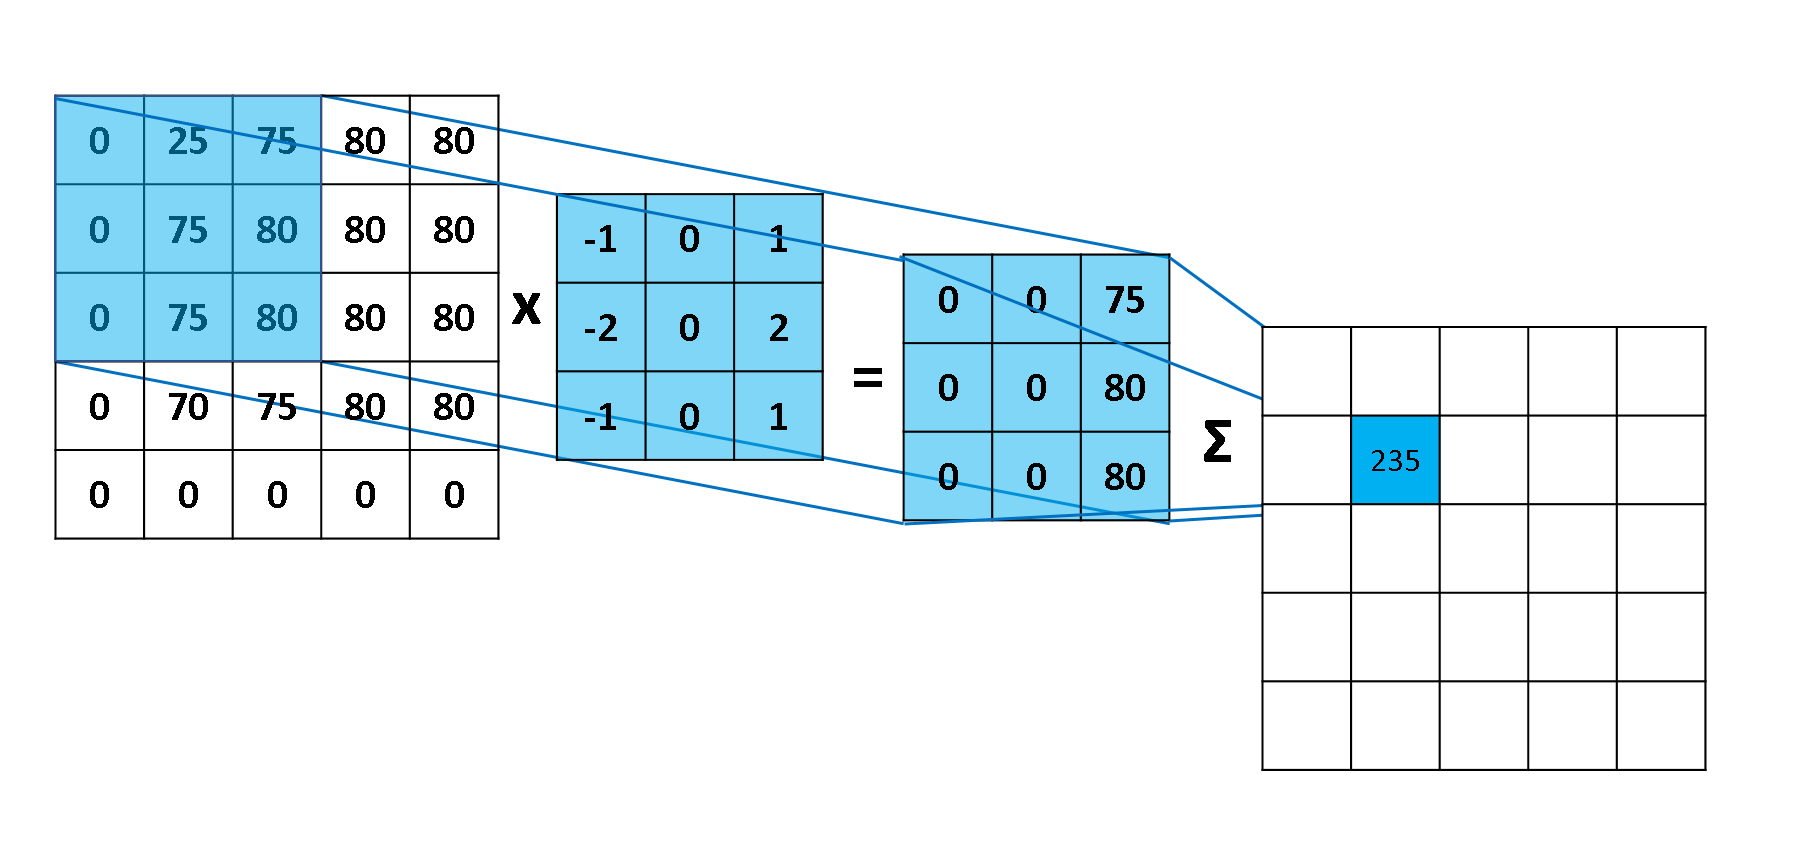
\includegraphics[width=.9\linewidth]{images/convolution.png}
\caption{\label{fig:convolution}Convolution step\autocite{ConvolutionalNeuralNetworks}}
\end{figure}

A convolutional neural network (CNN) is comprised of layers of 2D convolutions.
These layers consist of filters which themselves are comprised of kernels, small matrices with learned weights as values\autocite{osheaIntroductionConvolutionalNeural2015}.
Filters have a kernel for each input channel to the layer, with each kernel moving accross the channel and performing an elementwise multiplication with the part of the input it is currently on (Figure \ref{fig:convolution}).
The results of all kernels in a filter are summed into a single output pixel, meaning that each filter produces one output channel.
The stride of the layer determines how far the filter moves over the data every convolution, therefore a stride greater than one reduces the spatial dimensions by a factor of the stride size\autocite{dumoulinGuideConvolutionArithmetic2018}.
The inverse is also true, a sub-pixel stride of less than one increases the spatial dimensions, however this can lead to checkerboard artifacts where kernels overlap so a more appropriate technique is to interpolate the image into a larger size and then convolve over it, referred to as a resize-convolution\autocite{odenaDeconvolutionCheckerboardArtifacts2016}\autocite{aitkenCheckerboardArtifactFree2017}

\begin{figure}[htbp]
\centering
\includegraphics[width=.9\linewidth]{images/convolution_filter.png}
\caption{\label{fig:convolution_filter}Visualised convolution filters, with increasing complexity of features extracted\autocite{graetzHowVisualizeConvolutional2019}}
\end{figure}

Each kernel is unique, with the values of the matrix being the weights learned by through training.
Filters have a bias, which gets added to all values in the output data.
By using multiple filters with a stride greater than 1, the number of output channels can be increased whilst the spatial dimensions of the data is decreased.
This is a fundamental pattern in a CNN, as it allows for kernels to learn to extract features.
By reducing the spatial dimensions of the image, earlier layers extract low level features which get combined by following layers (Figure \ref{fig:convolution_filter}).
The compression of the input data also allows for later kernels to extract patterns from an area much larger than their kernel size .
Dilated convolutions expand the kernel by inserting holes between its elements, allowing the kernel to cover a larger area than its size\autocite{dumoulinGuideConvolutionArithmetic2018}.


\begin{figure}[htbp]
\centering
\includegraphics[width=.9\linewidth]{images/autoencoder.png}
\caption{\label{fig:autoencoder}Simplified diagram of an autoencoder\autocite{birlaAutoencoders2019}}
\end{figure}

\textbf{Autoencoders}

Autoencoders construct an encoder and decoder out of convolutional layers, using the change in channel number and spatial dimensions to learn to deconstruct then reconstruction data (Figure \ref{fig:autoencoder}).
The encoder is trained to reduce the spatial dimensions of the input data whilst increasing the number of channels.
The latent space is the result of this encoding, a lower-dimensional compressed representation of the data.
In a trained network, the latent space captures the most important features and patterns of the input data in a compact and efficient way\autocite{michelucciIntroductionAutoencoders2022}.
This representation is generalised, two different craters would be represented as craters, even if they had visual differences.
Autoencoders are useful for image inpainting as the latent space more clearly demonstrates the missing parts of features.
Dilated convolutions are especially effective in latent space, as the kernel acts over a larger area of the already compressed data for little computational cost, allowing it to learn complex and large features.
The decoder is trained to translate the latent space back into the inpainted image.
A famous use of autoencoders is in early "deepfake" networks, which are designed to swap faces in images.
In a deepfake network, separate autoencoders are trained for the two faces.
By swapping the decoder from one autoencoder into another, the autoencoder encodes properties (such face angle) for one face, however decodes the image with the other face.


\subsubsection{Generative Adversarial Networks}
\label{sec:org8dc4657}
Generative adversarial networks (GANs)\autocite{goodfellowGenerativeAdversarialNetworks2020} are a machine learning framework based on game theory.
They are constructed from two opposing networks, a generator and a discriminator.
The generator learns to generate fake data and attempts to trick the discriminator, which learns to distinguish between real and fake samples.
The adversarial loss between the competing networks is able to catch errors which would be overlooked by other loss functions, such as mean squared error\autocite{lotterUnsupervisedLearningVisual2016}.

A difficult challenge of training GANs is keeping the training of both generator and discriminator balanced.
If the discriminator becomes substantially better than the generator, the gradient for the generator will vanish as it is unable to ever trick the discriminator.
Wasserstein GANs\autocite{arjovskyWassersteinGenerativeAdversarial2017} (WGANs) improve this situation by using the Wasserstein-1 distance to measure discrepancy between real and generated data distributions, providing a stable and continuous gradient with a more meaningful relationship between the critics loss and the quality of the generated images.
In a WGAN, the discriminator is referred to as a critic as it learns to estimate the Wasserstein distance rather than simply classifying samples as real or fake, however its role is still adversarial as it competes with the generator to improve its estimate of the Wasserstein distance.
The Wasserstein-1 distance is also referred to as the Earth-Movers (EM) distance, as it is a measure of the minimum effort required to move one probability distribution into another.
To further improve the stability of the network, a gradient penalty can be applied to the network to ensure that the critic does not train too quickly and overpower the generator\autocite{gulrajaniImprovedTrainingWasserstein2017}.
If the gradient norm of the critic is too large, it is penalised to allow the generator to close the gap.

A GAN containing only convolutional layers is referred to as a deep convolutional GAN\autocite{radfordUnsupervisedRepresentationLearning2016}.
This simplification of the network is more computationally efficient than the GAN first proposed by Goodfellow et al.\autocite{goodfellowGenerativeAdversarialNetworks2020}, whilst allowing for deeper models and increased image resolution.
GANs typically use encoders and decoders, as novel data can be hallucinated in the latent space and then decoded to the output.
The addition of dilated convolutions\autocite{yuMultiScaleContextAggregation2016} as four layers in the latent space adds an enhanced receptive field, allowing for improved feature learning.

GAN training is unsupervised, meaning that it the training data set does not need to be labeled.
This is because data is known to be real or generated, and so the loss function can operate independently.
As training neural networks requires large amounts of data, unsupervised training requires far less human effort to achieve.
GANs are well suited for the task of void infilling, as the adversarial loss results in the generator being trained to generate the accurate DEMs, without the need of manually labeling voids locations.

\begin{figure}[htbp]
\centering
\includegraphics[width=.9\linewidth]{images/contextual_attention.png}
\caption{\label{fig:contextual_attention}Contextual attention focusing network on cat \autocite{zhangAgileAmuletRealTime2018}}
\end{figure}

\textbf{Contextual Attention}

Image features are extracted in convolutional neural networks with local kernels layer by layer.
This locality reduces the kernels effectiveness at borrowing from distant spatial locations; there may be many layers of convolutions reducing image spatial dimensions before data from other parts of the image become relevant to a kernel.
Yu et al.\autocite{yuGenerativeImageInpainting2018} proposed a novel contextual attention layer in the deep generative network to remedy this issue.
This layer learns where to copy feature information from in the known background (non-masked part of the image) to generate missing patches (Figure \ref{fig:contextual_attention}).
This concept is inspired by human attention, people selectively attend to specific aspects of the the environment based on relevance or saliency.
As the layer is differentiable it can be trained, improving the efficiency of the network as a whole.
The fully-convolutional nature of the contextual attention layer results in it being highly effective in image inpainting GANs; by matching background regions to copy from the network does not have to hallucinate entirely novel data, with the resulting inpainting result being more cohesive with the rest of the image.

\subsection{Related Work}
\label{sec:org12533ca}

\emph{A Neural Process Approach for Probabilistic Reconstruction of No-Data Gaps in Lunar Digital Elevation Maps} by Park and Choi\autocite{parkNeuralProcessApproach2021} is the most relevant work to this paper, as it also attempts to solve the issue of lunar DEM void reconstruction.
They use a sparse attentive neural processes (SANPs) (a novel implementation of attentive neural processes\autocite{kimAttentiveNeuralProcesses2019}) to reduce complexity and prevent over-fitting.
This works on a similar concept to the contextual attention layer proposed by Yu \emph{et al.}\autocite{yuGenerativeImageInpainting2018} and used in the current paper; training the network to identify regions in the input image that are more or less important for the infilling task.
Due to being fully convolutional in nature, contextual attention layers are likely more effective at improving void infilling GANs, with strong inpainting results described by Yu \emph{et al.}

A problem of void infilling GANs is that whilst a trained GAN produces plausible output data, it is impossible to asses the data accuracy, severely hampering the ability to use this data in future scientific missions.
To overcome this issue, Park and Choi implement uncertainty analysis in their void filling network.
This produces uncertainty maps of infilled regions, which indicate how confident the network is of each pixel.
Whilst the network proposed in the current paper likely produces more accurate void infilling results than Park and Choi - due to the use of contextual attention and slope data - uncertainty maps make infilled data more useful in real life applications.
In future work, uncertainty analysis could be implemented in the network described in this paper.

\emph{Void Filling of Digital Elevation Models With Deep Generative Models} by Gavriil \emph{et al.}\autocite{gavriilVoidFillingDigital2019} shares a similar network architecture to the current paper, as both are based on the inpainting network described by Yu \emph{et al.}\autocite{yuGenerativeImageInpainting2018}.
In the latent space of both the coarse and fine generators Gavriil \emph{et al.} added local feature extraction (LFE) layers for improved local feature aggregation.
Not only do other papers dispute the effectiveness of this\autocite{zhangVoidFillingBased2020}, LFE is designed to improve the networks efficiency with input data containing a high density of small objects at high resolution (50cm/pixel)\autocite{hamaguchiEffectiveUseDilated2018}, which is not such a relevant issue on the lunar surface.
In the current paper a technique is employed that is likely more effective in the context of lunar DEMs; small objects on the lunar surface such as boulders are highlighted to the network as the slope at the edges of the object is significantly greater than the surrounding terrain, and are not of a very high density.
The use of LFE layers likely makes the network described by Gavriil \emph{et al.} more effective at inpainting human structures such as cities, however the use of slope in the current paper is more suited for lunar DEMs.
To tackle the issue of a visible boundary at the edge of the infilled void, Gavriil \emph{et al.} implemented a custom algorithm which by solving for a best fitting paraboloid blended this region.
Whilst this was an effective technique, it is unnecessarily complex when compared to the poisson blending\autocite{perezPoissonImageEditing2003} implemented by the current paper.

In \emph{DEM Void Filling Based on Context Attention Generation Model} Zhang \emph{et al.}\autocite{zhangVoidFillingBased2020} makes the argument that the use of local feature extraction by Gavriil \emph{et al.}\autocite{gavriilVoidFillingDigital2019} has a negative impact on the networks ability to recover overall DEM semantic information.
Zhang \emph{et al.} also based their network architecture on the inpainting GAN described by Yu \emph{et al.}\autocite{yuGenerativeImageInpainting2018}, with the difference in opinion resulting in Zhang \emph{et al.} using an un-modified version of the network.
For void boundary post-processing,  Zhang \emph{et al.} used bilateral filtering, however poisson blending is more appropriate as DEM gradient information is preserved, whereas bilateral filtering is a lossy smoothing algorithm and so important data may be lost in the process.
The network also does not include the slope of the DEMs, so whilst it is built on the same network architecture as the current paper, it is likely less effective at preserving DEM texture.

\emph{Filling Voids in Elevation Models Using a Shadow-Constrained Convolutional Neural Network} by Dong \emph{et al.}\autocite{dongFillingVoidsElevation2020} introduces an additional loss function to train the network to adhere to geometric constraints implied by cast shadows.
This is achieved by extracting shadow maps from satellite imagery of the DEM location, which in combination with known sun directions are used to compute a shadow-based supervisory signal.
Whilst this may be an effective technique on earth, the requirement of cast shadows on the Moon poses an issue, as half of the moon is in permanent darkness.
The model described by Dong \emph{et al.} is a convolutional encoder-decoder, not a GAN.
GANs have been proven to solve the problem of insufficient data\autocite{nandhiniabiramiDeepCNNDeep2021}, making them more suited for void infilling than CNNs.

The terrain texture generation model (TTGM) described by Qui \emph{et al.} in \emph{Void Filling of Digital Elevation Models with a Terrain Texture Learning Model Based on Generative Adversarial Networks}\autocite{qiuVoidFillingDigital2019} served as the inspiration for using slope data in the void infilling network described by the current paper.
Elevation, terrain slope and relief degree (a measure of the maximum change in elevation in the 3x3 window around each pixel) composed the samples in the training set, allowing the network to learn more complex terrain texture than by just training on elevation.
TTGM was tested using simulated voids of a realistic shape and was able to capture deep features of the DEM data and structural patterns, including texture.
Whilst this was proven effective by Qui \emph{et al.}, the current paper found that including relief degree was expensive in terms of computation and memory usage; for little improvement.
Relief degree data is largely similar to the slope of a pixel, as pixels with a high relief degree will in turn likely have a large slope.
By removing relief degree from the training set, memory equal to the size of the DEM elevation training data was freed, and the initial pre-processing stage became faster.

TTGM also uses a deep convolutional GAN (DCGAN), however of a different architecture than the one described by the current paper.
Instead of featuring an autoencoder, TGGM has a symmetrical GAN structure, where the generator and critic are the same structure inverted.
Although TTGM uses Wasserstein distance, it does not feature a contextual attention layer, encoder-decoder architecture, coarse and fine generators or local and global critics and so whilst both use slope data, the network described by the current paper is likely more effective at DEM void infilling, whilst being more efficient in terms of memory.
Both networks use resize-convolutions\autocite{aitkenCheckerboardArtifactFree2017}\autocite{odenaDeconvolutionCheckerboardArtifacts2016} to remove checkerboard artifacts from convolutional layers that increase spatial dimensions.
Qui \emph{et al.} were the only authors to use batch normalisation within the generator of their network.

Two different models of input sizes 64x64 and 128x128 were trained by Qui \emph{et al.}, to adapt to different sizes of voids.
They proposed a multi-scale void filling strategy in which tiles are divided into differently sized patches depending on the size of the voids, with the appropriate network used for infilling.
These patches would then be joined to form a seamless infilled DEM.
This technique could be applied to the network described in the current paper, as Qui \emph{et al} note that the network trained with smaller input sizes has more accurate infilling results, however is limited to the size of void it can infill.

Gavriil \emph{et al.}, Zhang \emph{et al.}, Dong \emph{et al.} and Qui \emph{et al.} all trained their respective networks on DEM data from the Earth.
Whilst this means that the trained models would not be effective at lunar void infilling, lunar and earth DEM data is functionally the same and so the same network architecture could be used for lunar void infilling if trained on lunar DEMs.


\section{Methodology}
\label{sec:org68d4ee8}

\subsection{Problem Formation and Notation}
\label{sec:org6d6cde2}

Due to the similar nature of the problem being solved, the problem notation has been adapted from Gavriil \emph{et al.}\autocite{gavriilVoidFillingDigital2019}.
DEMs in both GeoTiff, PDS3 and PDS4 will be considered, in all of which data forms a grid with a single height value for every position \((i, j)\).
Let \(D = (d_p) \in \mathbb{R}^{m \times n}\) be a partial matrix of elevation values, where \(p\) is an abbreviation for pixel referring to the coordinates \((i,j)\) of a point on the DEM grid and \(d_p\) is the corresponding height value.
Also let \(S = (s_p) \in \mathbb{R}^{m \times n}\) be a partial matrix of the slope values of \(D\), where \(s_p\) is the corresponding slope at pixel \(p\).
Partial meaning that some pixel values are considered void.
A binary matrix \(M = (m_p) \in 0,1^{m \times n}\) acts as a mask representing the void regions of \(D\) and \(S\).
We refer to pixels \(p\) for which \(m_p = 1\) as \emph{known}, and \emph{unknown} otherwise.

\textbf{Problem}: Given an initial partial elevation model \(D^0\), slope of the elevation model \(S^0\), construct a complete elevation model \(D\) with semantically plausible generated values for the masked regions.



\subsection{Data Pre-Processing}
\label{sec:orga6a1b76}

\textbf{Need to add a graph of data pipeline}

\begin{figure}[htbp]
\centering
\includegraphics[width=.9\linewidth]{images/compression.png}
\caption{\label{fig:compression}DEM before and after tiling and removing null values}
\end{figure}

The python library GDAL\autocite{rouaultevenGDAL2023} was used for the loading and saving of DEM data from disk, which was then converted to NumPy\autocite{NumPy} arrays for pre-processing, before finally being converted into PyTorch\autocite{PyTorch} tensors for training.

As DEMs are raster data, each pixel in a square grid must have a stored value, even if that value is null (Figure \ref{fig:compression} (a)).
The data is tiled into 256x256 tiles for use in network training (Algorithm \ref{alg:tiling}), with tiles containing null values discarded before training begins.
This is memory inefficient and increases the data loading time before training can begin, however the main issue became apparent when uploading for cloud training, as this unnecessary data increases upload time and in tern cost.
To remedy this issue, each DEM file was compressed by initially tiling and discarding tiles containing null values, then saving back to a GeoTiff (Figure \ref{fig:compression} (b)).
The compressed file can only ever be tiled at the same size as when it was initially compressed, however this suited the requirements of this paper and reduced the size of the training data from 12.4GB to 8.1GB.
It is worth noting that this compression is lossy, any tile which contains even 1 null pixel is discarded.
A more data efficient technique may be an optimisation algorithm, which attempts to fit the maximum number of tiles into the irregular shape of the DEM, however this would add significant computational complexity and there was more than enough DEM data available for training.

\begin{algorithm}

\DontPrintSemicolon

\SetKwInOut{KwIn}{Input}
\SetKwInOut{KwOut}{Output}

\caption{Tiling Algorithm}
\label{alg:tiling}

\KwIn{2D array of DEM elevation values $D[1..m][1..n]$, $tileHeight$, $tileWidth$}
\KwOut{3D array of DEM tiles}

\uIf{$m \Mod{tileHeight} \neq 0$}{
    $newHeight \gets m - (m \Mod{tileHeight})$ \;
    $D \gets D[:newHeight]$ \tcp*[f]{Array slicing}\;
}
\ElseIf{$n \Mod{tileWidth} \neq 0$}{
    $newWidth \gets n - (n \Mod{tileWidth})$ \;
    $D \gets D[:][:newWidth]$ \tcp*[f]{Array slicing}\;
}

$tilesHigh \gets \lfloor\frac{m}{tileHight}\rfloor$ \;
$tilesWide \gets \lfloor\frac{n}{tileWidth}\rfloor$ \;

$tiledArray \gets D.reshape(tilesHigh, tileHight, tilesWide, tileWidth)$  \tcp*[f]{Change array stride}\;
$tiledArray \gets tiledArray.swapaxes(1,2)$ \;

$tiledArray \gets tiledArray.reshape(tilesHigh * tilesWide, tileHight, tileWidth)$ \;

\KwRet{$tiledArray$}

\end{algorithm}

Each DEM file contained within the data directory is loaded with GDAL, converted into a NumPy array and then tiled using Algorithm \ref{alg:tiling}.
The slope of each tile was calculated using the NumPy \texttt{gradient} function, which used the same formula as Equation \ref{eqn:slope},whilst being written in C instead of python so improving pre-processing speeds by a considerable margin.

It is important for input data into a neural network to be normalised for a number of reasons.
In the context of DEMs, pixels with a greater elevation value would cause greater activations in the input layer of the network, so an input tile at the top of a hill would be weighted greater than one at the bottom of a crater.
There is also theoretically no limit to the elevation value of a pixel, and so this massive potential range in training data values makes it very difficult for the network to learn patterns.
Data normalisation solves this issue by normalising all input data individually to between a certain range.
The range for the network described in this paper is between -1 and 1, as the network outputs data in the same range and so by storing the minimum and maximum values of a DEM tile, the tile can be de-normalised after infilling.
It is important to note that for a tile, elevation values and slope values must be normalised independently of each other.
For each tile, data is normalised using the following equation:

Let \(T\) be a matrix with values equal to the DEM tile of size \(m \times n\)
\begin{equation}\label{eq:normalise}
normalised = 2\left(\frac{T - min(T)}{max(T) - min(T)}\right) - 1
\end{equation}

After each file has been tiled, slope calculated and then normalised, it is appended to a linked list and then the next file is processed.
Once the final tile has been processed, all tiled DEM arrays in the linked list are combined into one large NumPy array.
While this is very memory inefficient, as twice the memory is required whilst the data is copied into the NumPy array, the alternative would require calculating the tiled size of each DEM before processing and then copying into a pre-allocated NumPy array, which was not within the scope of this project.
The NumPy array is then converted to a PyTorch tensor, however this is computationally very cheap as both use the same representation of n-dimensional arrays in memory and so does not involve copying.

A threading pool was originally implemented to increase the speed of pre-processing, as most of work is handled by external C libraries which are not limited by the fact that only one python thread can execute bytecode at a time.
Despite success in reducing loading times, the issue of pre-processing memory usage became considerably worse and longer load times were judged to be preferable over higher memory usage.


\subsection{Deep Generational Model}
\label{sec:orgb9ca196}

\subsubsection{Deep Generational Model Structure}
\label{sec:org643cc87}

The proposed DEM void infilling model is an adaptation of the image inpainting model proposed by Yu \emph{et al.}\autocite{yuGenerativeImageInpainting2018}.
This GAN architecture consists of a two-stage coarse to fine generator (Figure \ref{fig:generator}) which increases the receptive fields of the convolutional layers and two critics (Figure \ref{fig:critic}).
The generator \(G\) takes as input DEM elevation and slope with void pixels set equal to 1, and a binary mask to indicate the hole regions, outputting infilled elevation and slope values.
Input data is of the size 256x256 and has a random rectangular void, sometimes splitting the entire DEM to simulate DEM joining tasks.
The coarse network is trained explicitly with spatially discounted reconstruction loss, whereas the refinement network is trained with spatially discounted reconstruction loss plus two WGAN-GP losses, one critic judging the local loss of the inpainted area and a second the global loss of the entire infilled DEM;  enforcing consistency between infilled area and ground truth.
As both WGAN-GP and spatially discounted pixel-wise reconstruction losses measure \(l_1\) distances, the combined loss is more efficient and stable to train.
The reconstruction losses reward the autoencoders for taking a DEM with voids and reconstructing it to infill the voids.
As the coarse network takes as input the DEM with voids, it is much harder for it to learn to generate high level features, and so lower frequency data is generated.
The power of the refinement network is the re-prediction of rough generated values, giving it a more complete scene which enables its encoder to learn better feature representation than the coarse network.

\begin{figure}[htbp]
\centering
\includegraphics[width=.9\linewidth]{images/critic_architecture.png}
\caption{\label{fig:critic}Critic Architecure}
\end{figure}

\begin{figure*}
\centering
\includegraphics[width=.9\linewidth]{images/gan_architecture.png}
\caption{\label{fig:generator}Generator Architecure}
\end{figure*}

On initial training attempts, a strong checkerboard pattern was apparent within the infilled voids (Figure \ref{fig:checkerboard}).
This would not be such an issue in image inpainting, as the subtle changes in color may be imperceivable to the eye, however the margin of error for a DEM is much lower when viewed in 3D.
Not only does this reduce the usefulness of the data, but also adds instability to the training of the network and makes it difficult to approach a local minimum.
Initially it was suspected that these checkerboards were the result of sub-pixel convolutions\autocite{aitkenCheckerboardArtifactFree2017}, however upon inspection it was discovered that the architecture described by Yu \emph{et al.} already makes use of resize-convolutions\autocite{odenaDeconvolutionCheckerboardArtifacts2016} to mitigate this.
Odena, \emph{et al.}\autocite{odenaDeconvolutionCheckerboardArtifacts2016} also attribute critics that use convolutional layers with a kernel size that is not divisible by the stride with checkerboard artifacts, and as the artifacts were not present at the beginning of training and steadily became worse it can be inferred that they were a learned behavior.
As the kernels of the critic convolutional layers overlapped on certain pixels, the generator learned to abuse this and lower GAN losses by generating DEMs which also followed this pattern.
The kernel sizes for critic convolutional layers were changed from 5 to 4, whilst no convolutions in the generator increase spatial dimensions, instead using nearest-neighbor interpolation.
The convolutional structure for the entire model can be viewed in Table \ref{table:convolutions}, where the critic convolutions are also listed.
In addition, batch normalisation was implemented in the critic to add noise to each batch, requiring the critic to learn more generalised patterns to adapt to the noise, preventing artifact patterns from compounding.

\begin{figure}[htbp]
\centering
\includegraphics[width=.9\linewidth]{images/checkerboard.png}
\caption{\label{fig:checkerboard}Checkerboard Artifacts}
\end{figure}

\begin{figure}[htbp]
\centering
\includegraphics[width=.9\linewidth]{images/bn_loss.png}
\caption{\label{fig:bn_wloss}Unstable wasserstein loss with batch normalisation}
\end{figure}

All of these changes resulted in a big improvement in the data output by the generator, however there were still some pattern artifacts appearing.
Initially to attempt to resolve this batch normalisation was introduced to all layer of the generators, except the input and output layers.
Yu \emph{et al.} did not use batch normalisation in their model as it is expensive in terms of VRAM and they found it to deteriorate color coherence.
As can be seen in Figure \ref{fig:bn_wloss}, batch normalisation lead to instability in the network, with the loss functions of the model showing no signs of decreasing whilst adding artifacts to the inpainted DEM.
This may be because in adversarial settings, batch normalisation reduces the inter-class margin (separation of learned high-level features), which when applied to a DEM infilling network which relies on training for a high inter-class margin, leads to the observed instability\autocite{kongWhyDoesBatch2023}.
To address the issue of these artifacts, an additional layer was added to the end of both generators, using a tanh activation function and relatively large kernel sizes (table 1).
Yu \emph{et al.} used no activation functions in the final layer of their generators, using the Pytorch \texttt{clip} function to compress output weights to between -1 and 1, however using tanh introduces non-linearity to the final layer and the large kernel sizes of the additional final layers allow the generator to learn to remove any artifacts which it generates.



\begin{table*}[htbp]
\caption{\label{table:convolutions}Details of network convolutions, (K)ernel, (S)tride, (C)hannels, (P)adding}
\centering
\begin{tabular}{rllll}
Layer & Coarse Generator & Fine Generator & Contextual Attention (CA) & Critics\\[0pt]
\hline
1 & K5,S1,C32,P2 & K5,S1,C32,P2 & K5,S1,C32,P2 & K4,S2,C64,P1\\[0pt]
2 & K3,S2,C64,P1 & K3,S2,C32,P1 & K3,S2,C32,P1 & K4,S2,C128,P1\\[0pt]
3 & K3,S1,C64,P1 & K3,S1,C64,P1 & K3,S1,C64,P1 & K4,S2,C256,P1\\[0pt]
4 & K3,S2,C64,P1 & K3,S2,C64,P1 & K3,S2,C128,P1 & K4,S2,C256,P1\\[0pt]
5 & K3,S1,C128,P1 & K3,S1,C128,P1 & K3,S1,C128,P1 & Fully connected to 1\\[0pt]
6 & K3,S1,C128,P1 & K3,S1,C128,P1 & K3,S1,C128,P1 & \\[0pt]
7 & K3,D2,S1,C128,P2 & K3,D2,S1,C128,P2 & K3,S1,C128,P1 & \\[0pt]
8 & K3,D4,S1,C128,P4 & K3,D4,S1,C128,P4 & CA Layer & \\[0pt]
9 & K3,D8,S1,C128,P8 & K3,D8,S1,C128,P8 & K3,S1,C128,P1 & \\[0pt]
10 & K3,D16,S1,C128,P16 & K3,D16,S1,C128,P16 & K3,S1,C128,P1 & \\[0pt]
11 & K3,S1,C128,P1 & Join with CA layer & Join with Fine Generator & \\[0pt]
12 & K3,S1,C128,P1 & K3,S1,C128,P1 &  & \\[0pt]
13 & Resize (2x) & K3,S1,C128,P1 &  & \\[0pt]
14 & K3,S1,C64,P1 & Resize (2x) &  & \\[0pt]
15 & K3,S1,C64,P1 & K3,S1,C64,P1 &  & \\[0pt]
16 & Resize (2x) & K3,S1,C64,P1 &  & \\[0pt]
17 & K3,S1,C32,P1 & Resize (2x) &  & \\[0pt]
18 & K3,S1,C16,P1 & K3,S1,C32,P1 &  & \\[0pt]
19 & K3,S1,C2,P1 & K3,S1,C16,P1 &  & \\[0pt]
20 & K5,S1,C2,P2 & K3,S1,C2,P1 &  & \\[0pt]
21 &  & K7,S1,C2,P3 &  & \\[0pt]
\end{tabular}
\end{table*}


\subsubsection{Wasserstein GAN Gradient Penalty Loss}
\label{sec:orgc15b3d5}

A Wasserstein GAN uses the \emph{Earth-Mover} (EM) distance \(W(\mathbb{P}_r \mathbb{P}_g)\), also known as the \emph{Wasserstein-1} distance instead of the KL divergence used by Goodfellow \emph{et al.}\autocite{goodfellowGenerativeAdversarialNetworks2020} in the initial GAN proposition.
The EM distance for the real data distribution \(\mathbb{P}_r\) and generated data distribution \(\mathbb{P}_g\)  is the minimum cost of transporting mass to convert \(\mathbb{P}_r\) to \(\mathbb{P}_g\).
It is mathematically defined as the greatest lower bound (infimum) for any transport plan \(\gamma\):

\begin{equation}
W(\mathbb{P}_r,\mathbb{P}_g) = \inf_{\gamma \in \Pi(\mathbb{P}_r,\mathbb{P}_g)} \mathbb{E}_{(x,y) \sim \gamma}\left[\Vert x - y \Vert \right]
\end{equation}
\(\Pi(\mathbb{P}_r, \mathbb{P}_g)\) denotes the set of all joint distributions \(\gamma(x,y)\) whose marginals are respectively \(\mathbb{P}_r\) and \(\mathbb{P}_g\).
\(\Pi\) contains all the possible transport plans.

Using the Kantorovich-Rubinstein duality, the calculation can be simplified to:
\begin{equation}
W(\mathbb{P}_r, \mathbb{P}_{g}) = \sup_{\Vert f \Vert L \leq 1} \mathbb{E}_{x \sim \mathbb{P}_r} \left[f(x)\right] - \mathbb{E}_{x \sim \mathbb{P}_{g}} \left[f(x)\right]
\end{equation}
Where \(sup\) is the least upper bound and \(f\) is a 1-Lipschitz function that follows the constraint:
\begin{equation}
\vert f(x_1) - f(x_2) \vert \leq \vert x_1 - x_2 \vert
\end{equation}

This means that to calculate the EM distance, a 1-Lipschitz function must be found.
The critic of the network is used as \(f\) to learn the 1-Lipschitz function which most accurately calculates the EM distance, with the following objective function proposed by Arjovsky \emph{et al.}\autocite{arjovskyWassersteinGenerativeAdversarial2017}:
\begin{equation}
 \min_G \max_{D \in \mathcal{D}} \mathbb{E}_{x \sim \mathbb{P}_r} \left[D(x)\right] - \mathbb{E}_{\tilde{x} \sim \mathbb{P}_g} \left[ D(\tilde{x}) \right]
\end{equation}
Where \(\mathcal{D}\) is the set of 1-Lipschitz functions and \(\mathbb{P}_g\) is the model distribution implicitly defined by \(\tilde{x} = G(z)\), with \(z\) being the input to the generator.

The objective function of a GAN is the adversarial loss function, where the generator tries to minimise the function and the critic tries to maximise it.
In this case the critic maximises the objective function by learning a 1-Lipschitz function which more accurately calculates the EM distance.

To enforce \(D\) to be a 1-Lipschitz function, a WGAN clips the maximum weight value in \(D\) to a range determined by the hyperparameter \(c\), which must be tuned.
Clipping introduces problems such as vanishing gradients, with the original WGAN paper noting it was a terrible way to enforce a Lipschitz constraint\autocite{arjovskyWassersteinGenerativeAdversarial2017}.

Gulrajani \emph{et al.}\autocite{gulrajaniImprovedTrainingWasserstein2017} proposed an improved version of WGAN, using a gradient penalty (WGAN-GP) term instead of clipping to remedy these issues.
The penalty term is added to equation x to obtain a new objective function:
\begin{equation}
\begin{split}
 \min_G \max_{D \in \mathcal{D}} &\  \mathbb{E}_{x \sim \mathbb{P}_r} \left[D(x)\right] \\  &- \mathbb{E}_{\tilde{x} \sim \mathbb{P}_g} \left[ D(\tilde{x}) \right] \\ &+ \lambda \mathbb{E}_{\hat{x} \sim \mathbb{P}_{\hat{x}}} \left[ \Vert \nabla_{\hat{x}}D(\hat{x}) \Vert_2 - 1 \right]^2
\end{split}
\end{equation}
Where \(\hat{x}\) is sampled from the straight line between points sampled from distribution \(\mathbb{P}_g\) and \(\mathbb{P}_r\).
Yu \emph{et al.}\autocite{yuGenerativeImageInpainting2018} note that this is because the gradient of \(D^*\) at all points \(\hat{x} = (1-t)x + t\tilde{x}\) on the straight line should point directly towards current sample \(\tilde{x}\), therefore \(\nabla_{\hat{x}}D^*(\hat{x}) = \frac{\tilde{x} - \hat{x}}{\Vert \tilde{x} - \hat{x} \Vert}\).

For DEM infilling, only void regions should be predicted, thus the gradient penalty should only be applied to pixels within voids.
Yu \emph{et al.} implemented this with multiplication of gradients and input mask \(m\):
\begin{equation}
\begin{split}
 \min_G \max_{D \in \mathcal{D}} &\ \mathbb{E}_{x \sim \mathbb{P}_r} \left[D(x)\right] \\ &- \mathbb{E}_{\tilde{x} \sim \mathbb{P}_g} \left[ D(\tilde{x}) \right] \\ &+ \lambda \mathbb{E}_{\hat{x} \sim \mathbb{P}_{\hat{x}}} \left[ \Vert \nabla_{\hat{x}}D(\hat{x}) \odot (1 - m) \Vert_2 - 1 \right]^2
\end{split}
\end{equation}

Where the mask value is 0 for missing pixels and 1 for elsewhere.
\(\lambda\) was set to 10 for the training of the network.


\subsubsection{Spatially Discounted Reconstruction Loss}
\label{sec:org27b6a90}

Pixel-wise \(l_1\) reconstruction loss calculates the absolute difference between the original and reconstructed DEM.
This is a useful metric by which to judge the accuracy of the reconstruction, however void infilling requires hallucinations of pixels and so there are likely feasible solutions that are quite different than the original DEM.
When this happens, strong enforcement of the reconstruction loss in plausible patches differing from the original DEM may mislead the training process.
Intuitively, hallucinated pixels that are close to the boundary of the void are much more likely to be similar to the original DEM than at the center of the void.
Yu \emph{et al.}\autocite{yuGenerativeImageInpainting2018} introduced spatially discounted reconstruction loss which uses this intuition so as to not penalise the network for generating plausible but untruthful data.
Using a weight mask \(M\) to denote void regions, the weight of each pixel in the mask is computed as \(\gamma^l\), with \(l\) being equal to the distance of the pixel to the nearest known pixel.
By using a value of \(\gamma\) less than 1, the closer a pixel is to the center of a void, the less the weight its \(l_1\) loss is given.

\begin{figure}[htbp]
\centering
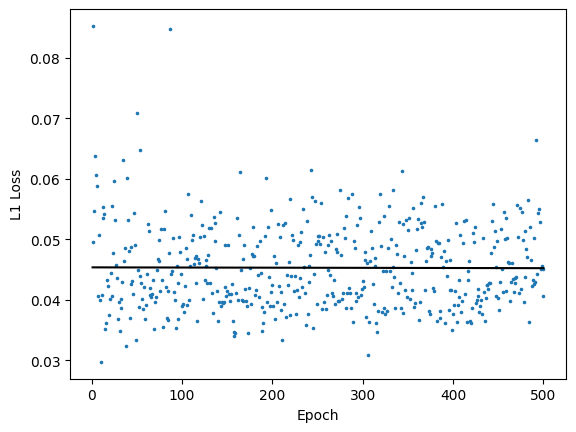
\includegraphics[width=.9\linewidth]{images/l1_loss.png}
\caption{\label{fig:l1_loss}Normal reconstruction loss}
\end{figure}

The effectiveness of spatially discounted reconstruction loss can be seen by comparing Figure \ref{fig:l1_loss} and Figure \ref{fig:ae_loss}.
Both graphs show their respective losses over training, with the spatially discounted reconstruction loss accurately showing convergence of the model around epoch 500 whilst the normal reconstruction loss has largely random values.
This must be taken in context, the network was not trained to minimise the normal reconstruction loss, however it demonstrates that plausible infilled data would have been penalised if using normal reconstruction loss.


\subsubsection{Contextual Attention Layer}
\label{sec:org0fd9245}
The contextual attention layer learns to copy features from known non-void patches into likely regions within a void, first described by Yu \emph{et al.}\autocite{yuGenerativeImageInpainting2018}.
For the purposes of the contextual attention layer, the non-void area is referred to as the background and the void area the foreground.
Patches are extracted from the background of size 3x3, and then reshaped as convolutional filters.
These background patches \(\left\{ b_{x^{\prime}, y^{\prime}} \right\}\) are matched with foreground ones \(\left\{ f_{x,y} \right\}\) to copy features to by measuring with normalised inner product:
\begin{equation}
s_{x,y,x^\prime,y^\prime} = \left \langle \frac{f_{x,y}}{\Vert f_{x,y} \Vert}, \frac{b_{x^\prime,y^\prime}}{\Vert b_{x^\prime,y^\prime} \Vert} \right \rangle
\end{equation}
Where \(s_{x,y,x^\prime,y^\prime}\) represents the similarity of feature matching between a patch centered in foreground \((x,y)\) and background \((x^\prime, y^\prime)\).

The attention score of each background block can be calculated with \(s^*_{x,y,x^\prime,y^\prime} = softmax_{x^\prime, y^\prime} \left( \lambda s_{x,y,x^\prime,y^\prime} \right)\), where \(\lambda\) is a constant value.
The optimal block \(\left \{ b_{x^\prime, y^\prime} \right\}\) is selected, and used as convolution filters to reconstruct foregrounds during deconvolution.
Values of overlapping pixels are averaged.
It can be inferred that matched patches will likely be coherent, meaning that a change in a background block will likely correspond to an equal change in a foreground block.
To help maintain the overall consistency of the infilled DEM, a left-right propagation is done, followed by a top-down propagation to get a new attention score for matched blocks.
For example, the equation for the left-right propagation for kernel size \(k\) is as follows:
\begin{equation}
\hat{s}_{x,y,x^\prime,y^\prime} = \sum_{i \in \{-k,\dots,k\}} s^*_{x,y,x^\prime,y^\prime}
\end{equation}

\subsubsection{Model Training}
\label{sec:org8bdfe28}

\autocite{yuGenerativeImageInpainting2018}
To integrate attention model, they introduce two parallel encoders as shown in figure x.
The bottom encoder specifically focuses on hallucinating contents with layer-by-layer (dilated) convolution, while the top one tries to attend on background features of interest.
Output features from two encoders are aggregated and fed into a single encoder to obtain the final output.


\emph{Me}
Contextual attention layer works thanks to the coarse network, so patches from the coarse network can be matched to patches of the background.


For training, given a raw image \(x\), we sample a binary image mask at a random location.
Input image \(z\) is corrupted from the raw image as \(z = x \odot m\).
Inpainting network \(G\) takes concatenation of \(z\) and \(m\) as input, and output predicted image \(x^\prime = G(z,m)\) with the same size as input.
Pasting the masked region of \(x^\prime\) to input image, we hey the inpainting output \(\tilde{x} = z + x^\prime \odot (1 - m)\).

Sample a batch of DEM tiles denoted as \(x\) randomly from the training data.
Random binary masks are generated for each tile in \(x\); with there being an equal chance that the masks are a normal rectangle or a rectangle which splits the tile vertically.
Input tiles \(z\) are corrupted from the ground truth \(x\) as \(z = x \odot m\).
Void infilling network \(G\) takes concatenation of \(z\) and \(m\) as input, with the output being the predicted tiles \(x^\prime = G(z,m\)).
\(x^\prime\) is the same size as the input tiles, however is entirely generated.
As the ground truth must not be edited in the final output, the infilled void regions of \(x^\prime\) are pasted into \(z\), with the final infilling result \(\tilde{x} = z + c^\prime \odot (1-m)\).

The critic is trained \(n\_critic\) times before training the generator once.
This ensures that the critic provides a more accurate estimation of the Wasserstein distance, leading to better and more stable training\autocite{arjovskyWassersteinGenerativeAdversarial2017}.
\(n\_critic\) was set to 5 for all training in this paper, as is usually the case


\begin{algorithm}
\DontPrintSemicolon

\caption{Network Training}
\label{alg:training}

\While{$G$ has not converged}{
    \For{ $i=1, \dots, n\_critic$}{
        Sample batch DEM tiles $x$ from training data \;
        Generate random masks $m$ for $x$ \;
        Construct inputs $z \gets x \odot m$ \;
        Get predictions $\tilde{x} \gets z + G(z,m) \cdot (1 - m)$ \;
        Sample $t \sim U[0,1]$ and $\hat{x} \gets (1 - t)x + t\tilde{x}$ \;
        Update two critics with $x$, $\tilde{x}$ and $\hat{x}$
    }
    Sample batch DEM tiles $x$ from training data \;
    Generate random masks $m$ for $x$ \;
    Update infilling network $G$ with spatially discounted $l_1$ loss and two adversarial critic losses \;
}

\end{algorithm}


\subsection{Data Post-processing}
\label{sec:orgf6f53ca}
\subsubsection{Poisson Blending}
\label{sec:org8686e90}
Due to the similarity with images, image processing techniques can be applied to the DEMs.
In this paper, the technique of poisson seamless cloning\autocite{perezPoissonImageEditing2003} was used as a post processing step to remove any boundary between the infilled area and original DEM.

For vertical masks the tile must be padded.
\subsubsection{Gaussian Blur}
\label{sec:orgf30b89e}


\section{Experiments}
\label{sec:orgefea328}
\subsection{Model Training}
\label{sec:org36b9e82}
Talk about all the changes made to the network

To train the network, large quantities of high quality DEM data is required.
Originally 5m/pixel LOLA DEMs of the lunar south pole were selected, however these featured an unacceptable quantity of artifacts.
NAC DEMs were found to be of much higher quality at similar and greater resolutions.
64 NAC DEMs\autocite{LROCRDRProduct} representing a variety of lunar terrain features were selected at random for the training set, with a further 32 selected for testing and validation purposes.
\subsection{Model Testing Methodology}
\label{sec:org669dd0a}


Compare slope to no slope

\section{Results}
\label{sec:org15bc943}

\begin{figure}[htbp]
\centering
\includegraphics[width=.9\linewidth]{images/ae_loss.png}
\caption{\label{fig:ae_loss}Spatially discounted reconstruction loss}
\end{figure}

AE loss is the spatially discounted reconstruction loss\autocite{zhangVoidFillingBased2020}

\begin{center}
\includegraphics[width=.9\linewidth]{images/wasserstein_loss.png}
\end{center}


\section{Discussion}
\label{sec:orgf8e3e15}

\section{Conclusion}
\label{sec:org5db1dd7}
Check if because the network is fully convolutional, can it be used on arbritrary sizes once trained
It is, so change related work section

\section{Future Work}
\label{sec:org8d51740}

Uncertainty maps
Maybe region normalisation?\autocite{yuRegionNormalizationImage2023}
Terrain texture based loss function

\section*{Acknowledgements}

\printbibliography

\section*{Appendices}
\end{document}